\let\negmedspace\undefined
\let\negthickspace\undefined
\documentclass[journal]{IEEEtran}
\usepackage[a5paper, margin=10mm, onecolumn]{geometry}
\usepackage{tfrupee}
\setlength{\headheight}{1cm}
\setlength{\headsep}{0mm}

\usepackage{gvv-book}
\usepackage{gvv}
\usepackage{cite}
\usepackage{amsmath,amssymb,amsfonts,amsthm}
\usepackage{algorithmic}
\usepackage{graphicx}
\usepackage{textcomp}
\usepackage{xcolor}
\usepackage{txfonts}
\usepackage{listings}
\usepackage{enumitem}
\usepackage{mathtools}
\usepackage{gensymb}
\usepackage{comment}
\usepackage[breaklinks=true]{hyperref}
\usepackage{tkz-euclide}
\usepackage{listings}

\def\inputGnumericTable{}
\usepackage[latin1]{inputenc}
\usepackage{color}
\usepackage{array}
\usepackage{longtable}
\usepackage{calc}
\usepackage{multirow}
\usepackage{hhline}
\usepackage{ifthen}
\usepackage{lscape}

\begin{document}

\bibliographystyle{IEEEtran}
\vspace{3cm}

\title{1.4.9m}
\author{EE24BTECH11017-D.KARTHIK}
\maketitle

\renewcommand{\thefigure}{\theenumi}
\renewcommand{\thetable}{\theenumi}
\setlength{\intextsep}{10pt}

\numberwithin{equation}{enumi}
\numberwithin{figure}{enumi}
\renewcommand{\thetable}{\theenumi}

\textbf{Question}:\\
Find the coordinates of the point which divides the line segment joining the points \( (1, -2, 3) \) and \( (3, 4, -5) \) in the ratio \( 2:3 \):
\begin{enumerate}
    \item internally, and
    \item externally.
\end{enumerate}

\solution:
Let \(\vec{A} = \myvec{1 \\ -2 \\ 3}\) and \(\vec{B} = \myvec{3 \\ 4 \\ -5}\). The ratio is \(m:n = 2:3\).

\begin{enumerate}
    \item \textbf{Internal Division:} \\
    The coordinates of the point dividing the line internally are given by:
    \begin{align}
    \vec{P} &= \frac{m\vec{B} + n\vec{A}}{m+n}\\
    &= \frac{2\myvec{3 \\ 4 \\ -5} + 3\myvec{1 \\ -2 \\ 3}}{2+3}\\
    &= \frac{\myvec{6 \\ 8 \\ -10} + \myvec{3 \\ -6 \\ 9}}{5}\\
    &= \frac{\myvec{9 \\ 2 \\ -1}}{5}\\
    \vec{P} &= \myvec{\frac{9}{5} \\ \frac{2}{5} \\ -\frac{1}{5}}
    \end{align}

    Therefore, the required point dividing the line internally is \(\myvec{\frac{9}{5} \\ \frac{2}{5} \\ -\frac{1}{5}}\).

    \item \textbf{External Division:} \\
    The coordinates of the point dividing the line externally are given by:
    \begin{align}
    \vec{Q} &= \frac{m\vec{B} - n\vec{A}}{m-n}\\
    &= \frac{2\myvec{3 \\ 4 \\ -5} - 3\myvec{1 \\ -2 \\ 3}}{2-3}\\
    &= \frac{\myvec{6 \\ 8 \\ -10} - \myvec{3 \\ -6 \\ 9}}{-1}\\
    &= \frac{\myvec{3 \\ 14 \\ -19}}{-1}\\
    \vec{Q} &= \myvec{-3 \\ -14 \\ 19}
    \end{align}

    Therefore, the required point dividing the line externally is \(\myvec{-3 \\ -14 \\ 19}\).
\end{enumerate}

\begin{figure}[h!]
   \centering
   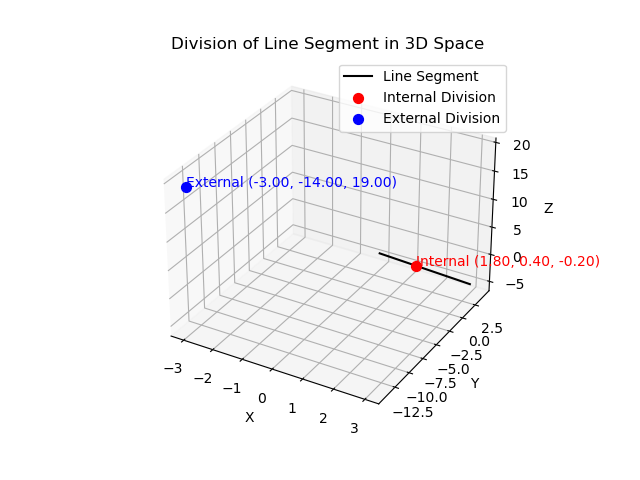
\includegraphics[width=0.7\linewidth]{figs/line_division.png}
   \caption{Internal and External Division of Line Segment}
\end{figure}

\end{document}
